\section{Implémentation de l'application web \\ \texttt{cognitivefactory-interactive-clustering-gui}}
\label{annex:C.3-DESCRIPTION-IMPLEMENTATION-INTERACTIVE-CLUSTERING-GUI}

	% INTRODUCTION DE L'ANNEXE.
	La librairie \texttt{cognitivefactory-interactive-clustering-gui} (\cite{schild-etal:2022:cognitivefactory-interactiveclusteringgui}) a été implémenté au cours de ce doctorat dans le but d'intégrer notre méthodologie de \texttt{Clustering Interactif} au sein d'une application web.
	Celle-ci dispose de plusieurs fonctionnalités telles que :
	\begin{itemize}
		\item la gestion du projet, de ses paramétrages et de ses données (cf. \textsc{Figures}~\textsc{\ref{figure:C-WEB-APPLICATION-LISTE-PROJETS}},~\textsc{\ref{figure:C-WEB-APPLICATION-ACCUEIL-PROJET}},~\textsc{\ref{figure:C-WEB-APPLICATION-PARAMETRAGE}} et~\textsc{\ref{figure:C-WEB-APPLICATION-INVENTAIRE-TEXTES}}) ;
		\item la gestion et l'annotation de contraintes, ainsi que la vérification des propriétés de transitivités (cf. \textsc{Figures}~\textsc{\ref{figure:C-WEB-APPLICATION-INVENTAIRE-CONTRAINTES}},~\textsc{\ref{figure:C-WEB-APPLICATION-ANNOTATION}} et~\textsc{\ref{figure:C-WEB-APPLICATION-CONFLIT}}) ;
		\item la gestion des étapes d'une itération et de l'exécution asynchrone des divers algorithmes (cf. \textsc{Figures}~\textsc{\ref{figure:C-WEB-APPLICATION-ACCUEIL-PROJET}} et~\textsc{\ref{figure:C-WEB-APPLICATION-DIAGRAMME-ETATS}}) ;
		\item quelques scripts d'analyses.
			% \footnote{Les scripts d'analyses concernent la visualisation des clusters et des composants connexes au cours des itérations, la vérification de la pertinence avec l'analyse des patterns linguistiques et les résumés automatiques de thématique, et l'analyse de la rentabilité avec l'évolution de la similarité entre résultats de \textit{clustering}.}.
	\end{itemize}
	
	Nous présenterons succinctement cette application ci-dessous à l'aide de captures d'écrans.
	
	% Information : comme y accéder.
	\begin{leftBarInformation}
		La documentation technique est accessible au lien suivant : \url{https://cognitivefactory.github.io/interactive-clustering-gui/}.
	\end{leftBarInformation}
	
	% Information : projet ingénieur TPS
	\setcounter{localCounterOfFootnoteValue}{\value{footnote}}
	\begin{leftBarInformation}
		L'étude d'une interface graphique et de ses fonctionnalités a été l'objet d'un premier projet étudiant avec l'école d'ingénieur Télécom Physique Strasbourg (au cours de l'année 2021).
		Lors de nos échanges, une idée consistait à s'inspirer des fonctionnalités de l'application \texttt{TINDER} \footnotemark pour \textit{swipe left} (respectivement \textit{swipe right}) l'annotation d'une contrainte \texttt{MUST-LINK} (respectivement d'une contrainte \texttt{CANNOT-LINK}).
		Bien qu'aucune version mobile de cette application n'a été développée, une telle fonctionnalité pourrait être envisagée afin d'améliorer le confort de l'utilisateur.
		On peut toutefois noter qu'un reliquat de cette discussion à mener au choix du logo de l'application, proche du logo de celui de l'application \texttt{TINDER}, ainsi qu'au design de la page d'annotation (cf. \textsc{Figure~\ref{figure:C-WEB-APPLICATION-ANNOTATION}}).
	\end{leftBarInformation}
		% Rattraper les footnote.
			\stepcounter{localCounterOfFootnoteValue}
			\footnotetext[\value{localCounterOfFootnoteValue}]{
				\url{https://tinder.com/fr}
			}
	
	% Note de l'auteur : en cours de maintenance.
	\begin{leftBarAuthorOpinion}
		Suite aux diverses études menées au cours de ce doctorat, certaines pages sont en cours de développement, notamment :
		\begin{itemize}
			\item les pages d'analyses dont le but d'intégrer les conclusions des \textsc{Section~\ref{section:4.4-HYPOTHESE-PERTINENCE}} et \textsc{Section~\ref{section:4.5-HYPOTHESE-RENTABILITE}} ;
			\item les pages de documentation pour intégrer les discussions du \textsc{Chapitre~\ref{chapter:5-GUIDE}}.
		\end{itemize}
	\end{leftBarAuthorOpinion}
	
	
	%%% Page d'accueil de l'application
	\newpage
	\paragraph{Page d'accueil de l'application (\textsc{Figure~\ref{figure:C-WEB-APPLICATION-ACCUEIL}}) :}
		
		% Capture d'écran: Page d'accueil de l'application.
		\begin{figure}[H]
			\centering
			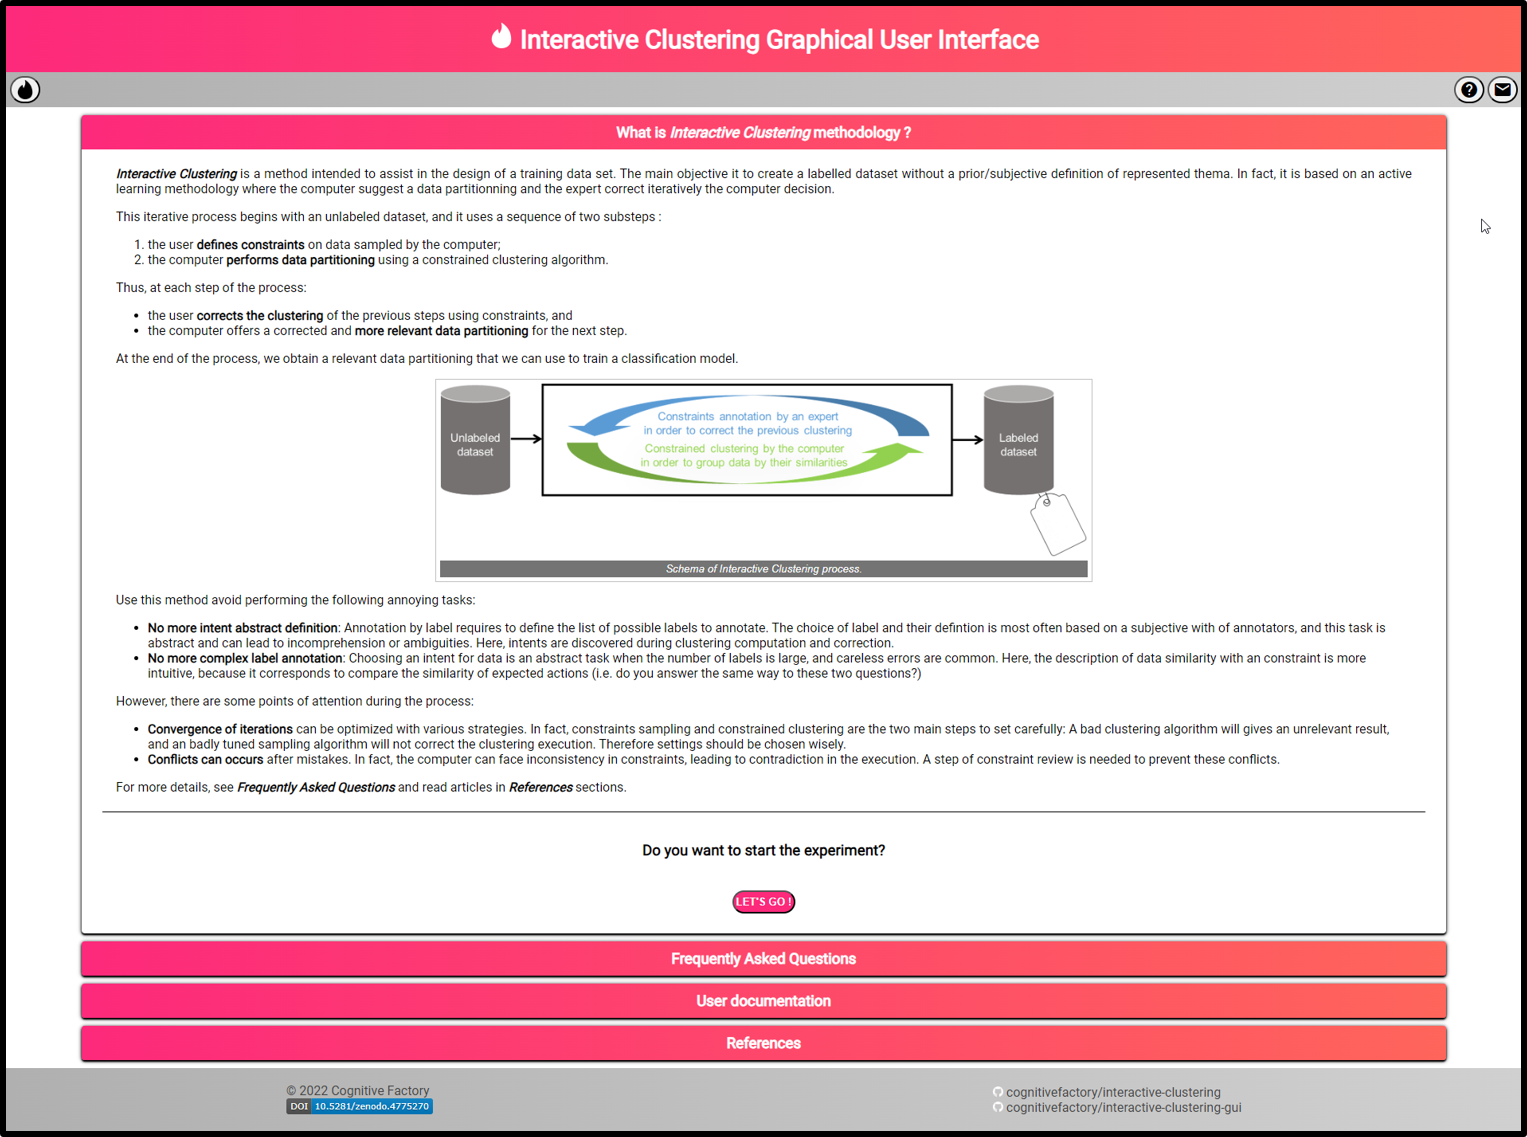
\includegraphics[width=0.95\textwidth]{figures/interactive-clustering-application-accueil-application}
			\caption{
				Capture d'écran de l'application web implémentant notre méthodologie de \texttt{Clustering Interactif} : \textbf{page d'accueil de l'application}.
			}
			\label{figure:C-WEB-APPLICATION-ACCUEIL}
		\end{figure}
		
		% Description générale.
		C'est la page de bienvenu de l'application.
		Nous y trouvons une description rapide de la méthode ainsi qu'une liste des questions fréquentes à son sujet.
		A terme, la documentation de la méthodologie d'annotation (cf. discussions du \textsc{Chapitre~\ref{chapter:5-GUIDE}}) y sera intégrée.
		
		% Boutons accessibles.
		Parmi les boutons accessibles, il y a :
		\begin{itemize}
			\item Le bouton d'accueil en haut à gauche, qui redirigera toujours sur cette page ;
			\item Le bouton de contact en haut à droite, qui permet de contacter l'équipe de recherche ;
			\item Le bouton \textguillemets{\texttt{LET'S GO}} qui permet d'accéder à la page de listant les projets d'annotation (cf. \textsc{Figure~\ref{figure:C-WEB-APPLICATION-LISTE-PROJETS}}).
		\end{itemize}
	
	
	%%% Page de gestion des projets
	\newpage
	\paragraph{Page de gestion des projets (\textsc{Figure~\ref{figure:C-WEB-APPLICATION-LISTE-PROJETS}}) :}
		
		% Capture d'écran: liste des projets.
		\begin{figure}[H]
			\centering
			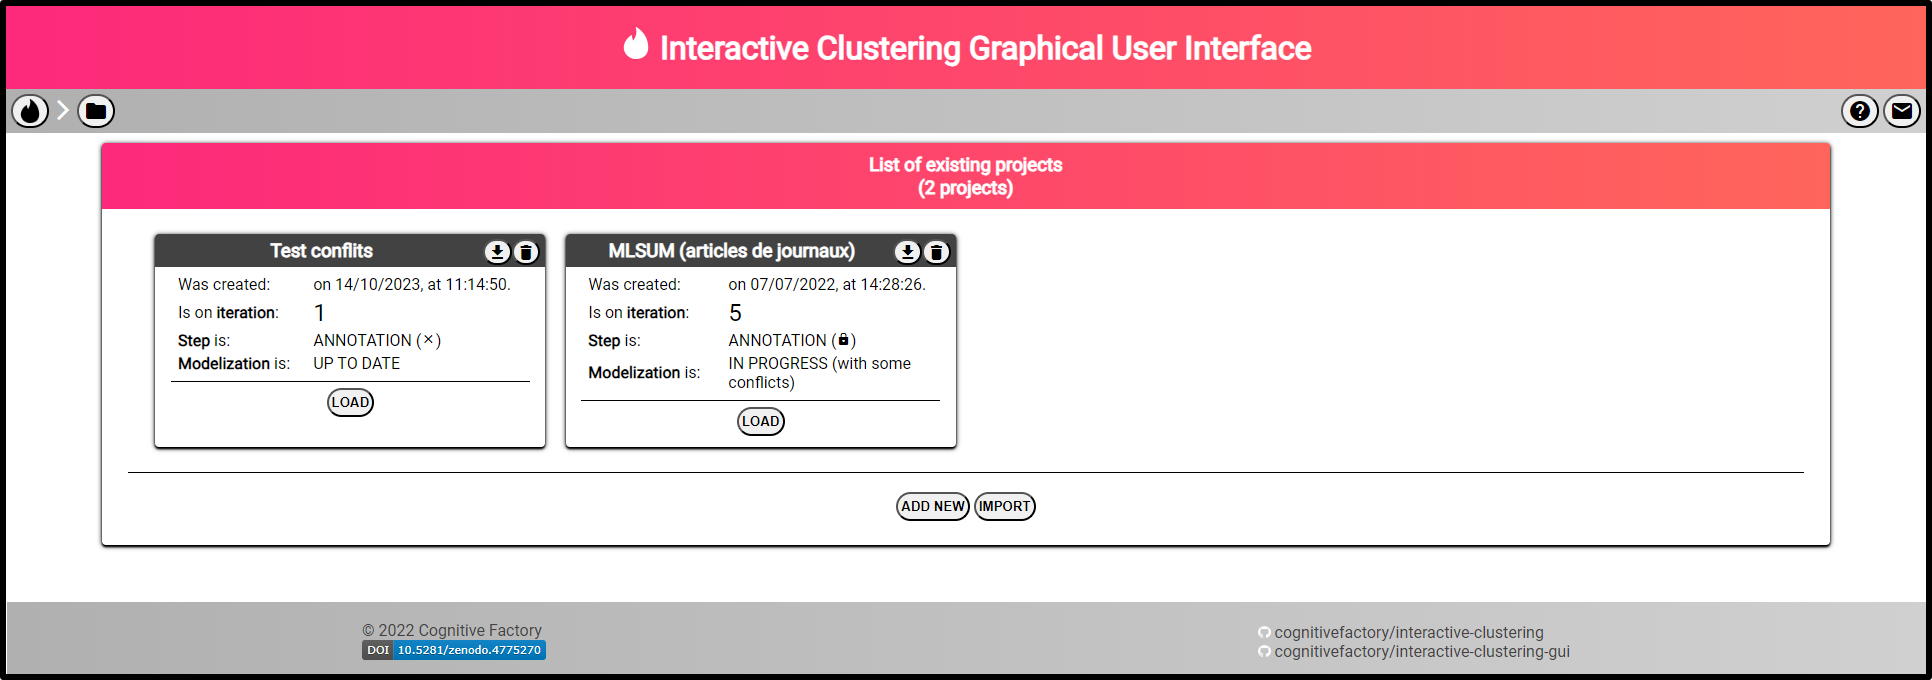
\includegraphics[width=0.95\textwidth]{figures/interactive-clustering-application-liste-projets}
			\caption{
				Capture d'écran de l'application web implémentant notre méthodologie de \texttt{Clustering Interactif} : \textbf{page de gestion des projets}.
			}
			\label{figure:C-WEB-APPLICATION-LISTE-PROJETS}
		\end{figure}
		
		% Description générale.
		Cette page liste les projets existants sous la forme de tuiles contenant les informations importantes : nom, date de création, nombre d'itérations de la méthode, et statut du projet (nous y reviendrons plus tard).
		
		% Boutons accessibles.
		\begin{itemize}
			\item Les boutons d'accueil en haut à gauche permettent de naviguer entre cette page et la page d'accueil de l'application (cf. \textsc{Figure~\ref{figure:C-WEB-APPLICATION-ACCUEIL}}) ;
			\item Il est possible de télécharger un projet au format \texttt{.zip} ou de le supprimer grâce aux boutons en haut à droite de chaque tuile ;
			\item Pour créer un projet, le bouton \textguillemets{\texttt{ADD NEW}} ouvre un formulaire demandant le nom du projet et la liste des textes à annoter (au format \texttt{.csv} séparateur '\texttt{;}') ;
			\item Il est aussi possible d'importer un projet contenu dans une archive \texttt{.zip} téléchargée au préalable grâce au bouton \textguillemets{\texttt{IMPORT}} ;
			\item Enfin, le bouton \textguillemets{\texttt{LOAD}} mène à la page d'accueil du projet sélectionné (cf. \textsc{Figure~\ref{figure:C-WEB-APPLICATION-ACCUEIL-PROJET}}).
		\end{itemize}
	
	
	%%% Page d'accueil du projet en cours
	\newpage
	\paragraph{Page d'accueil du projet en cours (\textsc{Figure~\ref{figure:C-WEB-APPLICATION-ACCUEIL-PROJET}}) :}
		
		% Capture d'écran: accueil projet.
		\begin{figure}[H]
			\centering
			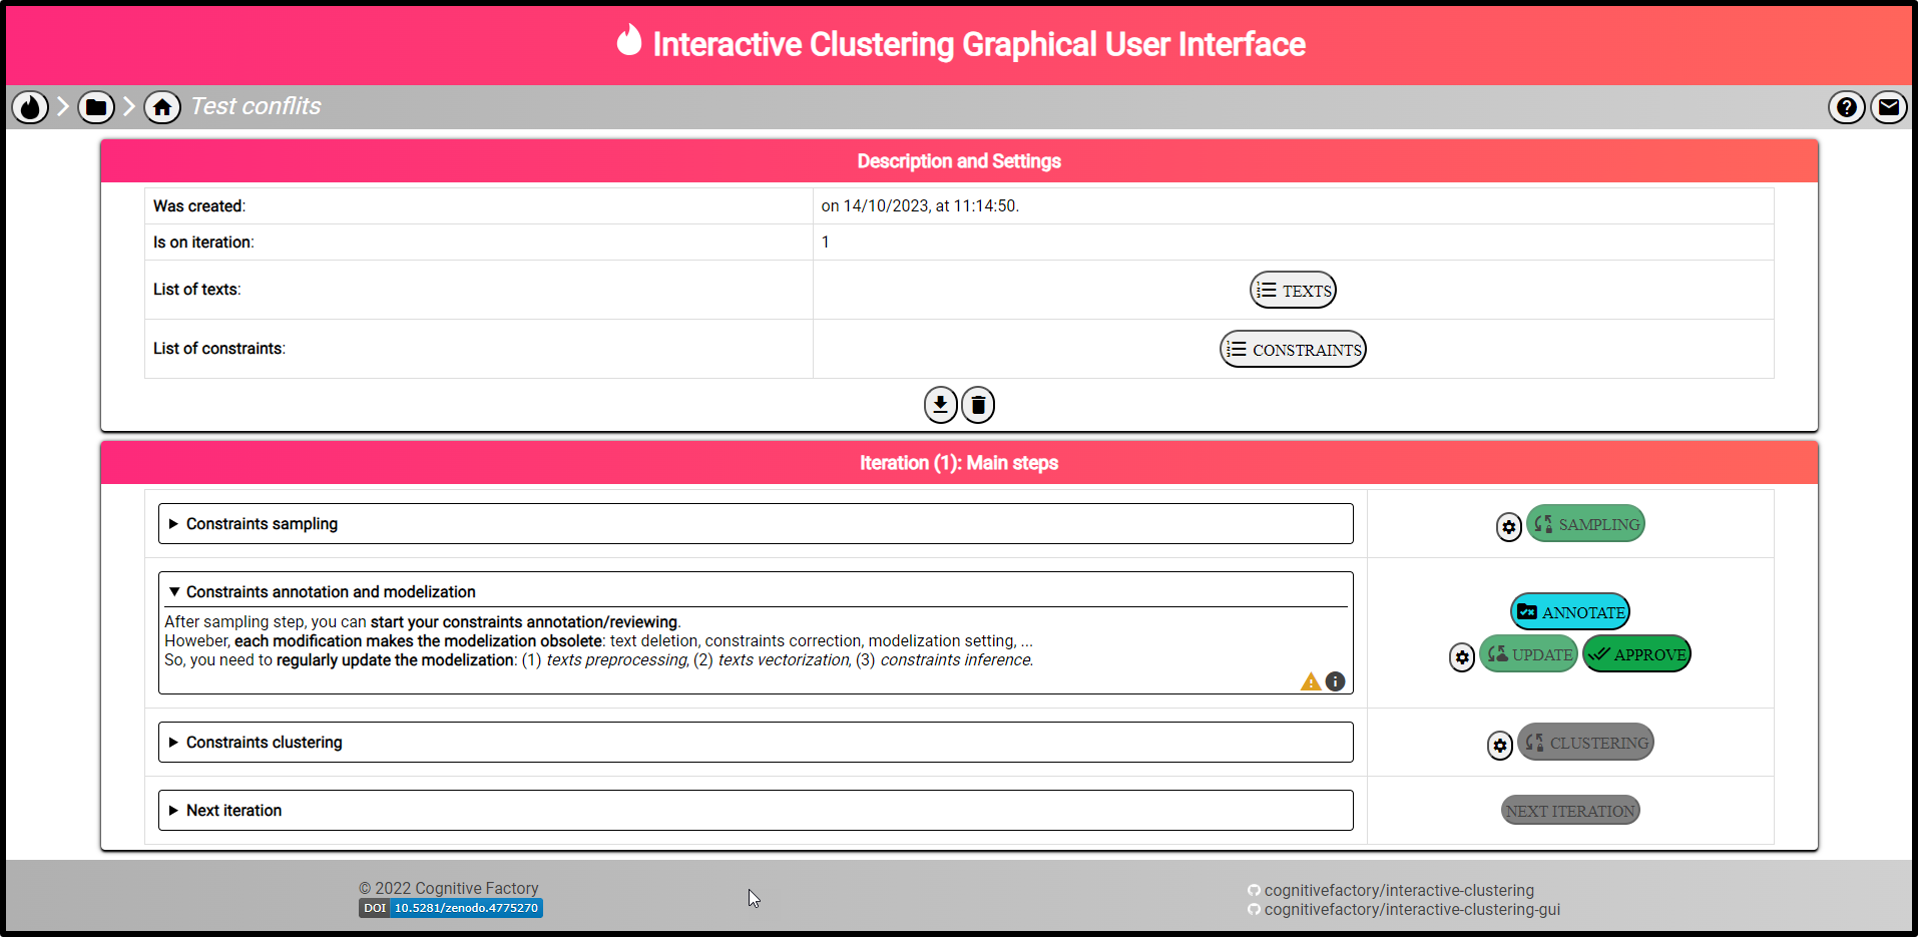
\includegraphics[width=0.95\textwidth]{figures/interactive-clustering-application-accueil-projet}
			\caption{
				Capture d'écran de l'application web implémentant notre méthodologie de \texttt{Clustering Interactif} : \textbf{page d'accueil du projet en cours}.
			}
			\label{figure:C-WEB-APPLICATION-ACCUEIL-PROJET}
		\end{figure}
		
		% Description générale.
		C'est la page principale de l'application. Elle contient en partie supérieure les informations du projet d'annotation en cours (\textit{date de création, numéro d'itération, gestion des données et des contraintes}), et en partie inférieure les étapes d'une itération de \texttt{Clustering Interactif} (\textit{description des étapes, boutons d'actions et de paramétrages}).
		
		% Boutons accessibles: gestion de projet.
		Concernant la gestion du projet (partie supérieure) :
		\begin{itemize}
			\item Les boutons d'accueil en haut à gauche permettent de naviguer entre cette page, la page de gestion des projets (cf. \textsc{Figure~\ref{figure:C-WEB-APPLICATION-LISTE-PROJETS}} et la page d'accueil de l'application (cf. \textsc{Figure~\ref{figure:C-WEB-APPLICATION-ACCUEIL}}) ;
			\item Au centre, il est possible de télécharger le projet au format \texttt{.zip} ou de le supprimer ;
			\item Le bouton \textguillemets{\texttt{TEXTS}} mène vers la page d'inventaire et de gestion des données du projet (cf. \textsc{Figure~\ref{figure:C-WEB-APPLICATION-INVENTAIRE-TEXTES}}) ;
			\item Le bouton \textguillemets{\texttt{CONSTRAINTS}} mène vers la page d'inventaire et de gestion des contraintes annotées ou en cours d'annotation (cf. \textsc{Figure~\ref{figure:C-WEB-APPLICATION-INVENTAIRE-CONTRAINTES}}).
		\end{itemize}
		
		% Boutons accessibles: gestion d'une itération.
		Concernant la gestion d'une itération de \texttt{Clustering Interactif} (partie inférieure), les différentes étapes sont représentées de bas en haut à l'aide d’éléments descriptifs repliables et de boutons d'actions.
		Nous retrouvons quatre étapes :
		\begin{enumerate}
			\item l'échantillonnage de contraintes, exécuté en tâche de fond par le bouton \textguillemets{\texttt{SAMPLING}}, et dont les paramètres sont accessibles via le bouton en forme de roue crantée ;
			\item l'annotation de contraintes, avec le bouton \textguillemets{\texttt{ANNOTATE}} qui redirige vers la prochaine contrainte à annoter.
			Cette étape contient aussi une gestion de la modélisation, c'est-à-dire une vérification des prétraitements et de la vectorisation des données, mais aussi une vérification de la cohérence des contraintes par l'absence de conflits d'annotation : le bouton \textguillemets{\texttt{UPDATE}} permet de recalculer cette modélisation en tâche de fond et le bouton \textguillemets{\texttt{APPROVE}} permet de la fixer jusqu'à la fin de l'itération en cours ;
			\item l'\textit{clustering} sous contraintes, exécuté en tâche de fond par le bouton \textguillemets{\texttt{CLUSTERING}}, et dont les paramètres sont accessibles via le bouton en forme de roue crantée ;
			\item la confirmation du passage à la nouvelle itération, exécuté avec le bouton \textguillemets{\texttt{NEXT ITERATION}}.
		\end{enumerate}
		
		% Notes:
		Il est à noter que :
		\begin{itemize}
			\item Les éléments de gauche sont repliables : au chargement de la page, seul l'élément de l'étape en cours est déplié ;
			\item La gestion de l'itération se fait à l'aide d'un diagramme d'état (cf. \textsc{Figure~\ref{figure:C-WEB-APPLICATION-DIAGRAMME-ETATS}}) : celui-ci se manifeste par un code couleur et l'activation/désactivation des boutons.
		\end{itemize}
	
	
	%%% Diagramme d'états de l'application et gestion des exécutions asynchrones
	\newpage
	\paragraph{Diagramme d'états de l'application et gestion des exécutions asynchrones (\textsc{Figure~\ref{figure:C-WEB-APPLICATION-DIAGRAMME-ETATS}}) :}
		
		% Capture d'écran: accueil projet.
		\begin{figure}[H]
			\centering
			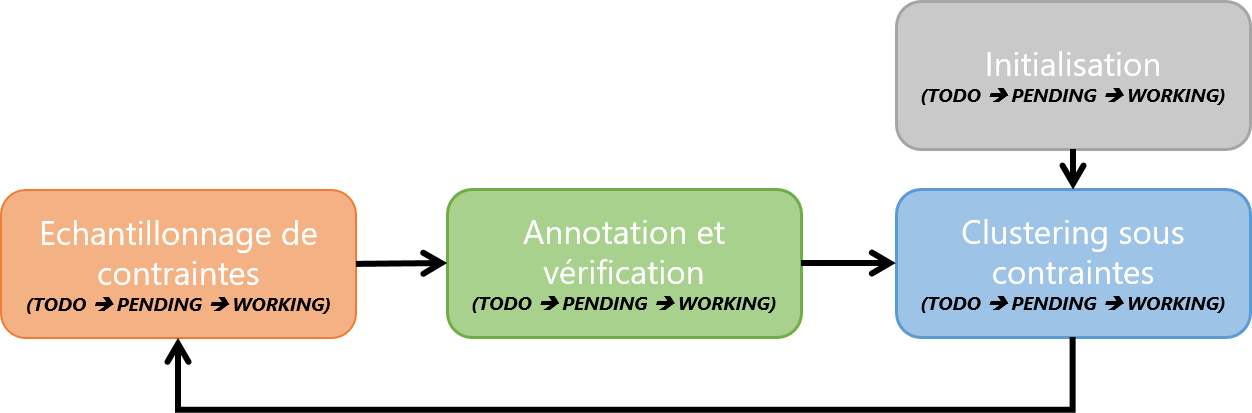
\includegraphics[width=0.95\textwidth]{figures/interactive-clustering-application-diagramme-etats}
			\caption{
				\textbf{Diagramme d'états} simplifié de l'application web implémentant notre méthodologie de \texttt{Clustering Interactif}.
			}
			\label{figure:C-WEB-APPLICATION-DIAGRAMME-ETATS}
		\end{figure}
		
		% Description générale.
		Comme décrit en \textsc{Section~\ref{section:3.2-DESCRIPTION-THEORIQUE}} et dans la \textsc{Figure~\ref{figure:3.2.1-DESCRIPTION-THEORIQUE-GENERALE}}, une itération de \textit{Clustering Interactif} contient trois étapes majeures : \textbf{(1)} l'échantillonnage de contraintes, \textbf{(2)} l'annotation de contraintes, et \textbf{(3)} le \textit{clustering} sous contraintes.
		Ces étapes sont représentés par le diagramme d'état en \textsc{Figure~\ref{figure:C-WEB-APPLICATION-DIAGRAMME-ETATS}} : ce dernier définit l'activation ou la désactivation des boutons d'action de l'application (cf. \textsc{Figure~\ref{figure:C-WEB-APPLICATION-ACCUEIL-PROJET}}).
		
		% Gestion de couleur.
		Afin de représenter l'état en cours et les actions possibles de manières pragmatique dans l'interface, un code couleur implicite est utilisé en plus de l'activation/désactivation des boutons :
		\begin{itemize}
			\item objet en \texttt{gris foncé} et généralement désactivé : action inaccessible pour le moment ;
			\item objet en \texttt{vert} et activé : prochaine action à réaliser ;
			\item objet en \texttt{cyan} : action en cours de traitement ;
			\item objet en \texttt{rouge} et activé : action en erreur ou à recommencer ;
			\item objet en \texttt{vert foncé} et généralement désactivé : action réalisée avec succès.
		\end{itemize}
		
		% Gestion des actions asynchrones.
		D'autre part, comme l'exécution de certains algorithmes peut être longue, ces derniers sont exécutées en tâche de fond.
		La gestion d'état est alors affinée en quatre sous-états :
		\begin{itemize}
			\item \texttt{TODO} : l'action est à faire, la machine attend l'ordre de l'utilisateur ;
			\item \texttt{PENDING} : l'action a été ordonnée par l'utilisateur, mais elle n'a pas encore été prise en charge en tâche de fond par la machine ;
			\item \texttt{WORKING} : l'action est en cours d'exécution en tâche de fond. Une barre d'avancement apparaît pour maintenir l'utilisateur informé de l'évolution de l'état ;
			\item Note: l'état \texttt{DONE} (action faite) est représentée par la prochaine étape avec un état \texttt{TODO}.
		\end{itemize}
		
		% Note: Architecture asynchrone en production.
		\begin{leftBarAuthorOpinion}
			Pour une simplicité d'usage et pour offrir une démonstration rapide, nous avons décider d'exécuter les algorithmes en tâche de fond.
			Toutefois, pour favoriser les performances de l'application et sa sûreté pour une utilisation en production, nous vous conseillons de réimplémenter cette gestion des exécutions en privilégiant une architecture asynchrone utilisant des \textit{workers} dédiés.
		\end{leftBarAuthorOpinion}
	
	
	%%% Page de gestion des paramètres
	\newpage
	\paragraph{Page de gestion des paramètres (\textsc{Figure~\ref{figure:C-WEB-APPLICATION-PARAMETRAGE}}) :}
	
		% Capture d'écran: gestion des paramètrages.
		\begin{figure}[H]
			\centering
			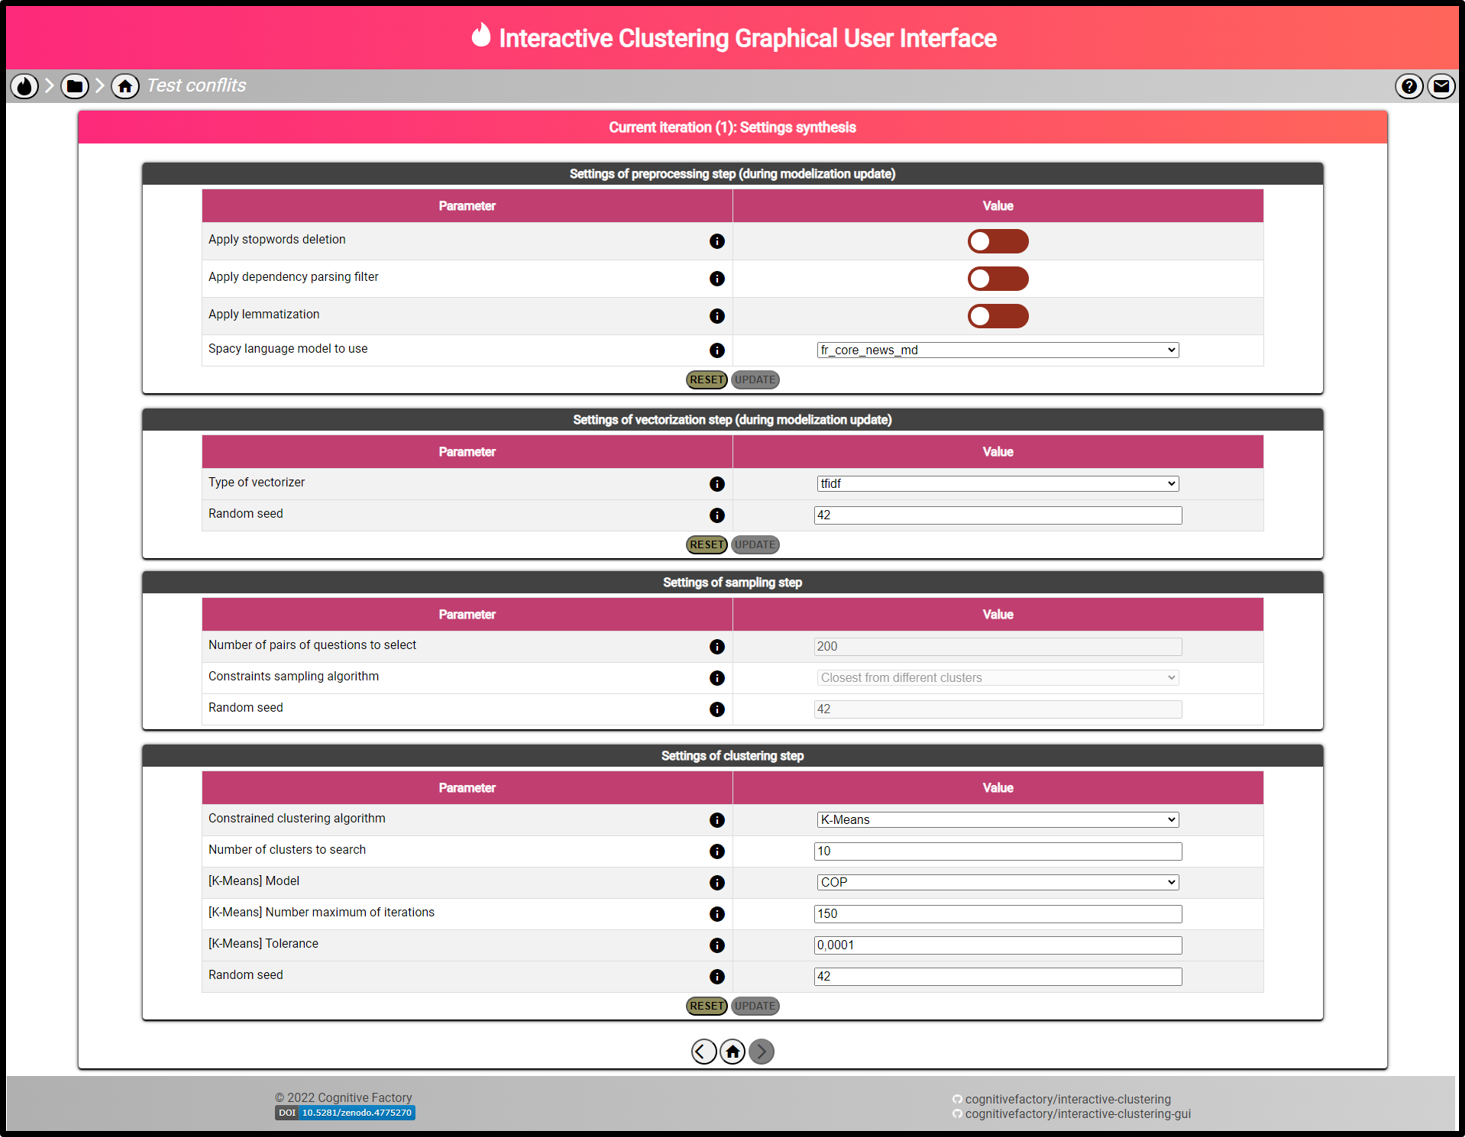
\includegraphics[width=0.95\textwidth]{figures/interactive-clustering-application-parametres}
			\caption{
				Capture d'écran de l'application web implémentant notre méthodologie de \texttt{Clustering Interactif} : \textbf{page de gestion des paramètres}.
			}
			\label{figure:C-WEB-APPLICATION-PARAMETRAGE}
		\end{figure}
		
		% Description générale.
		Accessible depuis les boutons en forme de roue crantée sur la page d'accueil du projet (cf. \textsc{Figure~\ref{figure:C-WEB-APPLICATION-ACCUEIL-PROJET}}), cette page liste les divers paramètres des algorithmes pour chaque itération.
		\begin{itemize}
			\item Chaque tuile représente un algorithme (prétraitements, vectorisation, échantillonnage et \textit{clustering}) : divers algorithmes et hyperparamètres son disponibles ;
			\item Ces différents formulaires sont modifiables tant que l'étape n'est pas en cours d'exécution, sinon ils sont juste consultables ;
			\item En bas de page, il est possible de changer d'itération pour consulter les paramètres des itérations précédentes et de revenir vers la page d'accueil du projet avec le bouton en forme de maison.
		\end{itemize}
	
	
	%%% Page d'inventaire des textes
	\newpage
	\paragraph{Page d'inventaire des textes (\textsc{Figure~\ref{figure:C-WEB-APPLICATION-INVENTAIRE-TEXTES}}) :}
	
		% Capture d'écran: inventaire des textes.
		\begin{figure}[H]
			\centering
			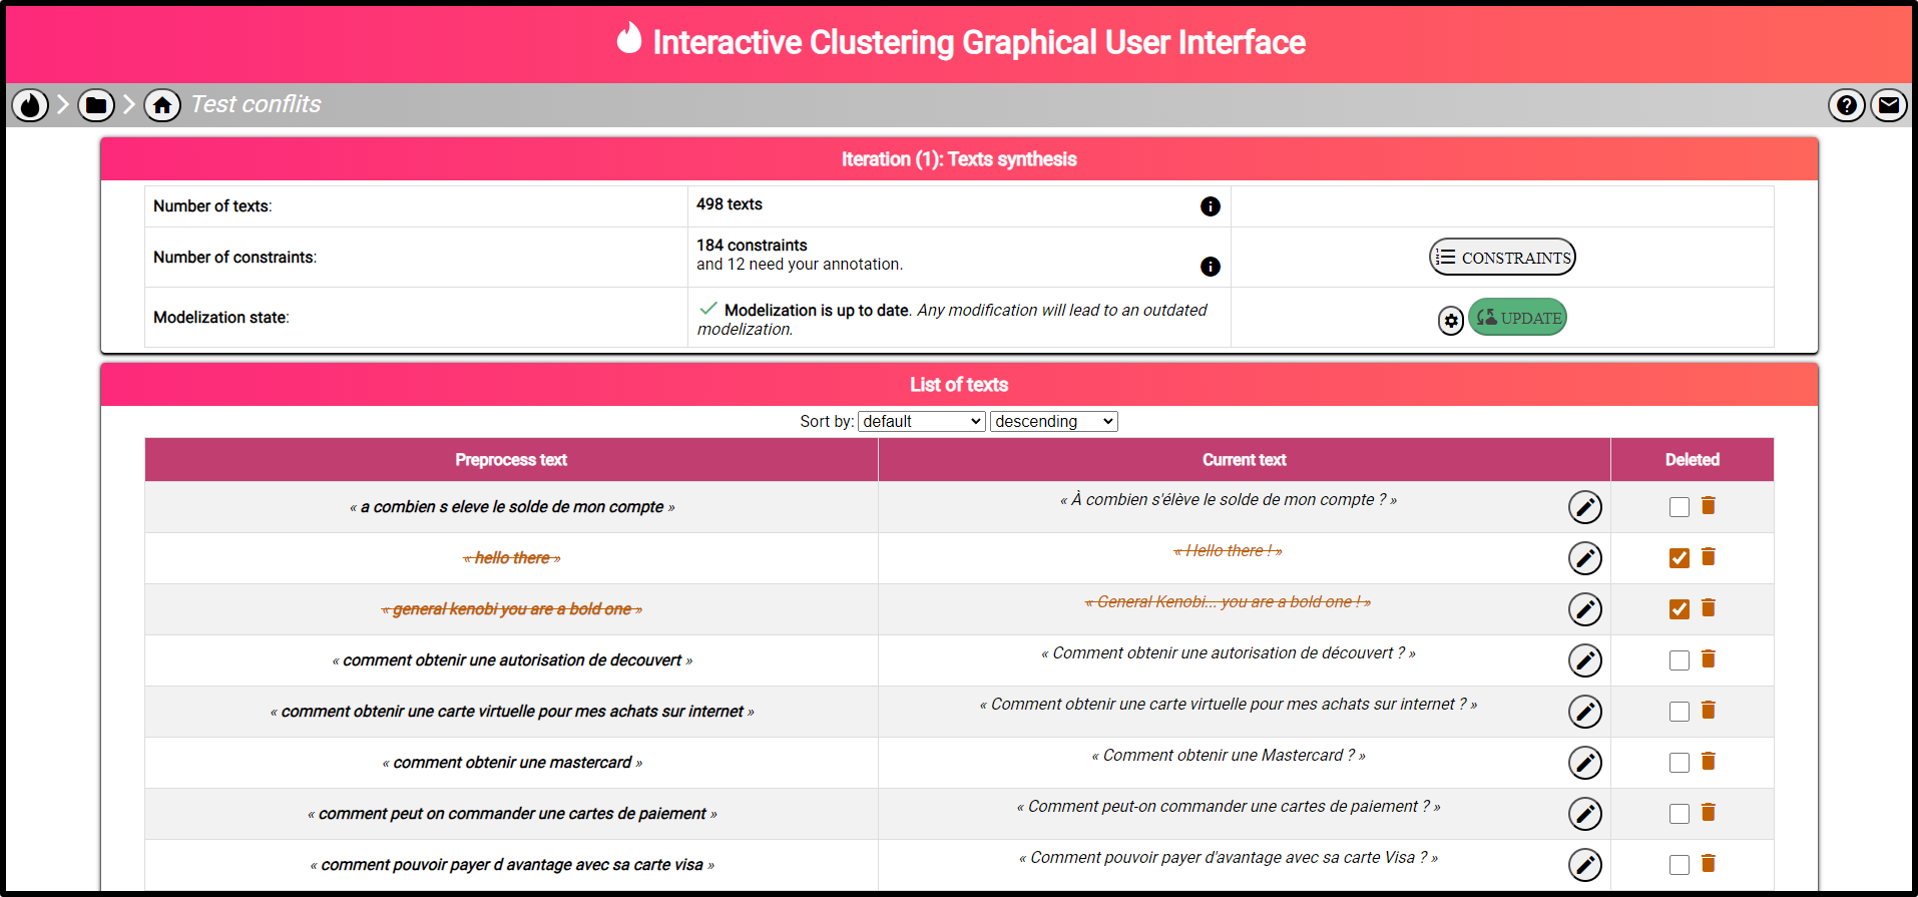
\includegraphics[width=0.95\textwidth]{figures/interactive-clustering-application-textes}
			\caption{
				Capture d'écran de l'application web implémentant notre méthodologie de \texttt{Clustering Interactif} : \textbf{page d'inventaire des textes}.
			}
			\label{figure:C-WEB-APPLICATION-INVENTAIRE-TEXTES}
		\end{figure}
		
		% Description générale.
		Cette page permet de lister les données du projet à annoter.
		La page est divisée en deux : la partie supérieure donne des informations générales (\textit{nombre de textes, nombre de contraintes à annoter, rappel de la modélisation en cours}), et la partie inférieure liste les textes dans un tableau.
		
		% Boutons accessibles: gestion des textes.
		Concernant les informations générales (partie supérieure) :
		\begin{itemize}
			\item Le bouton \textguillemets{\texttt{UPDATE}} permet de mettre à jour la modélisation si des contraintes ont été ajoutées, des paramètres de prétraitements ou de vectorisation ont été mis à jour ou si des textes ont été modifiés : cette action est exécutée en tâche de fond ;
			\item Le bouton \textguillemets{\texttt{CONSTRAINTS}} mène vers la page d'inventaire et de gestion des contraintes annotées ou en cours d'annotation (cf. \textsc{Figure~\ref{figure:C-WEB-APPLICATION-INVENTAIRE-CONTRAINTES}}).
		\end{itemize}
		
		% Boutons accessibles: liste des textes.
		Concernant le tableau listant les textes (partie inférieure) :
		\begin{itemize}
			\item Le texte brut et sa version prétraitée sont affichés ;
			\item Grâce bouton en forme de crayon, il est possible de corriger un texte s'il contient une faute de frappe.
			Une telle action nécessite de mettre à jour la modélisation par la suite ;
			\item Grâce à la coche en forme de poubelle, il est possible de supprimer un texte s'il n'est pas pertinent pour le projet : celui-ci est alors rayé en orange.
			Une telle action nécessite de mettre à jour la modélisation par la suite ;
			\item Les deux dernières actions sont désactivées si le projet n'est pas à l'étape d'annotation (cf. diagramme d'états en \textsc{Figure~\ref{figure:C-WEB-APPLICATION-DIAGRAMME-ETATS}}) ;
			\item Il est possible en haut du tableau de trier les textes suivant différents critères (\textit{ordre alphabétique, supprimé ou non, ...}).
		\end{itemize}
	
	
	%%% Page d'inventaire des contraintes
	\newpage
	\paragraph{Page d'inventaire des contraintes (\textsc{Figure~\ref{figure:C-WEB-APPLICATION-INVENTAIRE-CONTRAINTES}}) :}
	
		% Capture d'écran: inventaire des contraintes.
		\begin{figure}[H]
			\centering
			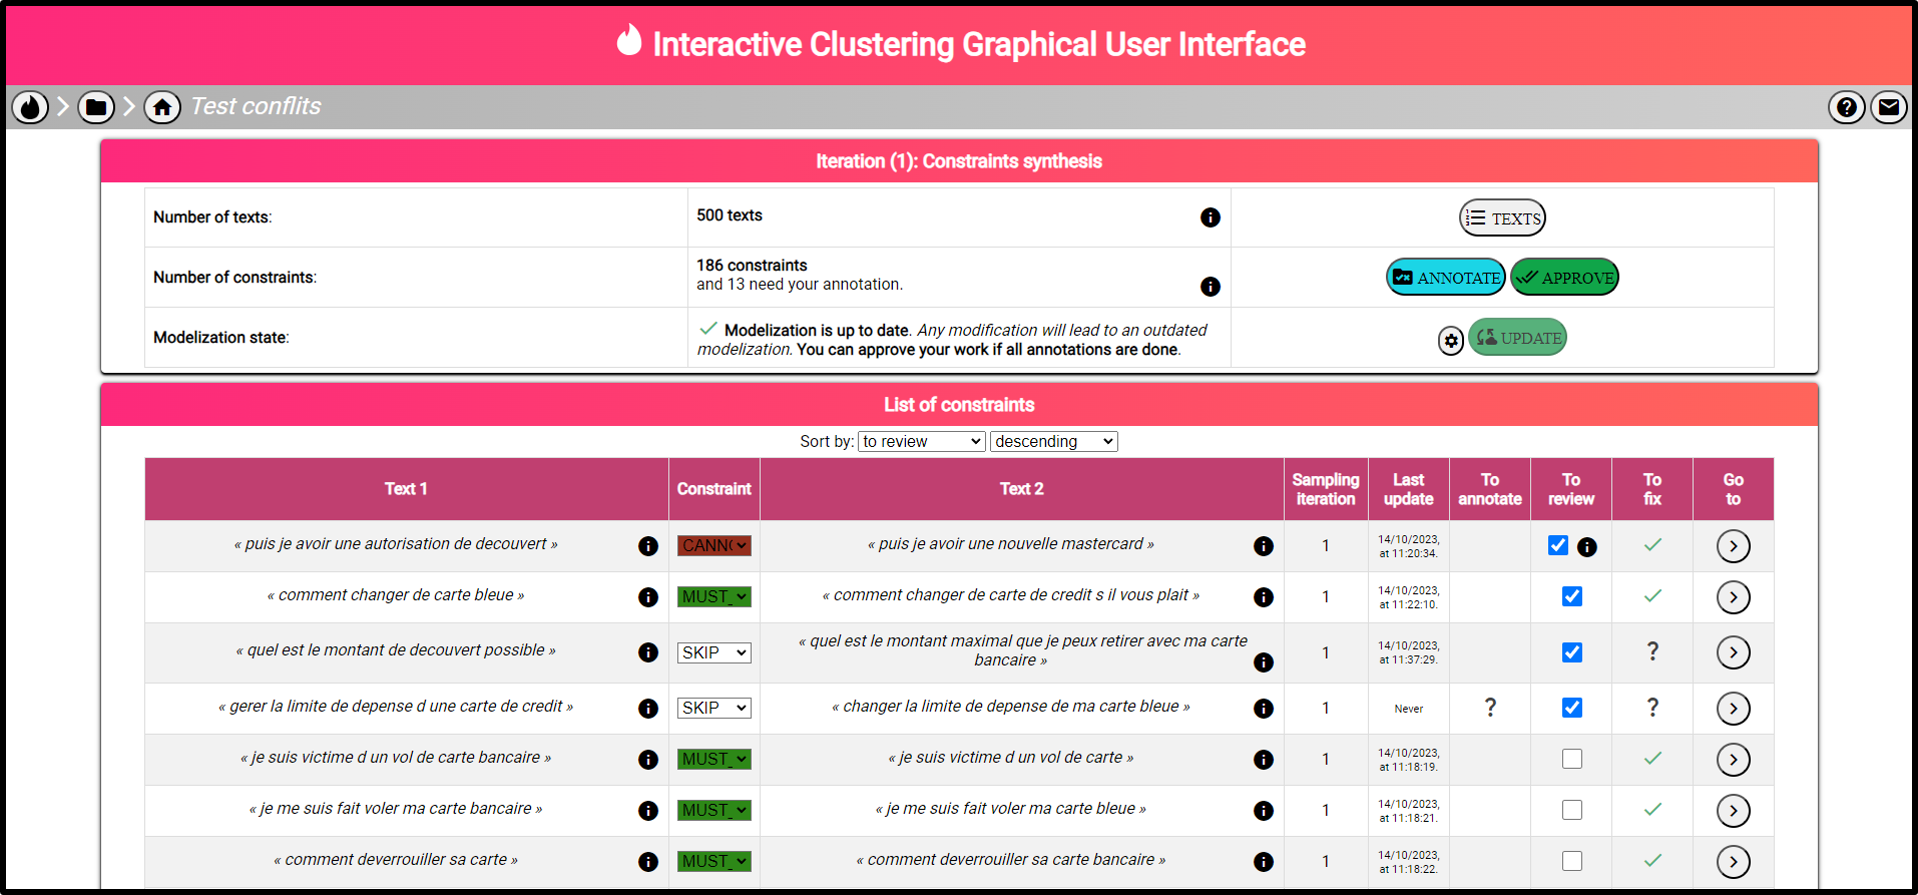
\includegraphics[width=0.95\textwidth]{figures/interactive-clustering-application-contraintes}
			\caption{
				Capture d'écran de l'application web implémentant notre méthodologie de \texttt{Clustering Interactif} : \textbf{page d'inventaire des contraintes}.
			}
			\label{figure:C-WEB-APPLICATION-INVENTAIRE-CONTRAINTES}
		\end{figure}
		
		% Description générale.
		Cette page permet de lister les contraintes du projet à annoter.
		La page est divisée en deux : la partie supérieure donne des informations générales (\textit{nombre de textes, nombre des contraintes à annoter, rappel de la modélisation en cours}), et la partie inférieure liste les contraintes dans un tableau.
		
		% Boutons accessibles: gestion des contraintes.
		Concernant les informations générales (partie supérieure) :
		\begin{itemize}
			\item Le bouton \textguillemets{\texttt{ANNOTATE}} redirige vers la prochaine contrainte à annoter (s'il en reste) ;
			\item Le bouton \textguillemets{\texttt{UPDATE}} permet de mettre à jour la modélisation si des contraintes ont été ajoutées, des paramètres de prétraitements ou de vectorisation ont été mis à jour ou si des textes ont été modifiés : cette action est exécutée en tâche de fond ;
			\item Le bouton \textguillemets{\texttt{TEXTS}} mène vers la page d'inventaire et de gestion des données du projet (cf. \textsc{Figure~\ref{figure:C-WEB-APPLICATION-INVENTAIRE-TEXTES}}).
		\end{itemize}
		
		% Boutons accessibles: liste des contraintes.
		Concernant le tableau listant les contraintes (partie inférieure) :
		\begin{itemize}
			\item Les deux textes d'une même contraintes sont affiché de part et d'autre de la valeur annotée : \texttt{MUST-LINK} en vert pour des données similaires, \texttt{CANNOT-LINK} en rouge pour des données différentes, \texttt{SKIP} en blanc pour une contrainte non-annotés ou temporairement ignorée ;
			\item La modification de la valeur annotée est désactivée si le projet n'est pas à l'étape d'annotation (cf. diagramme d'états en \textsc{Figure~\ref{figure:C-WEB-APPLICATION-DIAGRAMME-ETATS}}).
			Cette modification nécessite de mettre à jour la modélisation par la suite ;
			\item Il est possible de marquer une contraintes pour la revoir plus tard (coche bleue) ;
			\item Le bouton en forme de flèche à droite permet d'accéder à la page d'annotation de cette contrainte (cf. \textsc{Figure~\ref{figure:C-WEB-APPLICATION-ANNOTATION}}) ;
			\item Divers informations diverses sont disponibles à la droite du tableau : l'itération à laquelle la contrainte a été échantillonnée, sa dernière date de modification, son besoin d'annotation (\textit{un point d'interrogation veut dire que la contrainte n'a jamais été annotée}), et la présence ou non de conflit (\textit{coche verte ou point d'exclamation rouge}) ;
			\item Il est possible en haut du tableau de trier les contraintes suivant différents critères (\textit{ordre alphabétique, valeur d'annotation, date d'échantillonnage ou de modification, présence de conflit, ...}).
		\end{itemize}
	
	
	%%% Page d'annotation d'une contrainte
	\newpage
	\paragraph{Page d'annotation d'une contrainte (\textsc{Figure~\ref{figure:C-WEB-APPLICATION-ANNOTATION}} et \textsc{Figure~\ref{figure:C-WEB-APPLICATION-CONFLIT}}) :}
	
		% Capture d'écran: annotation.
		\begin{figure}[H]
			\centering
			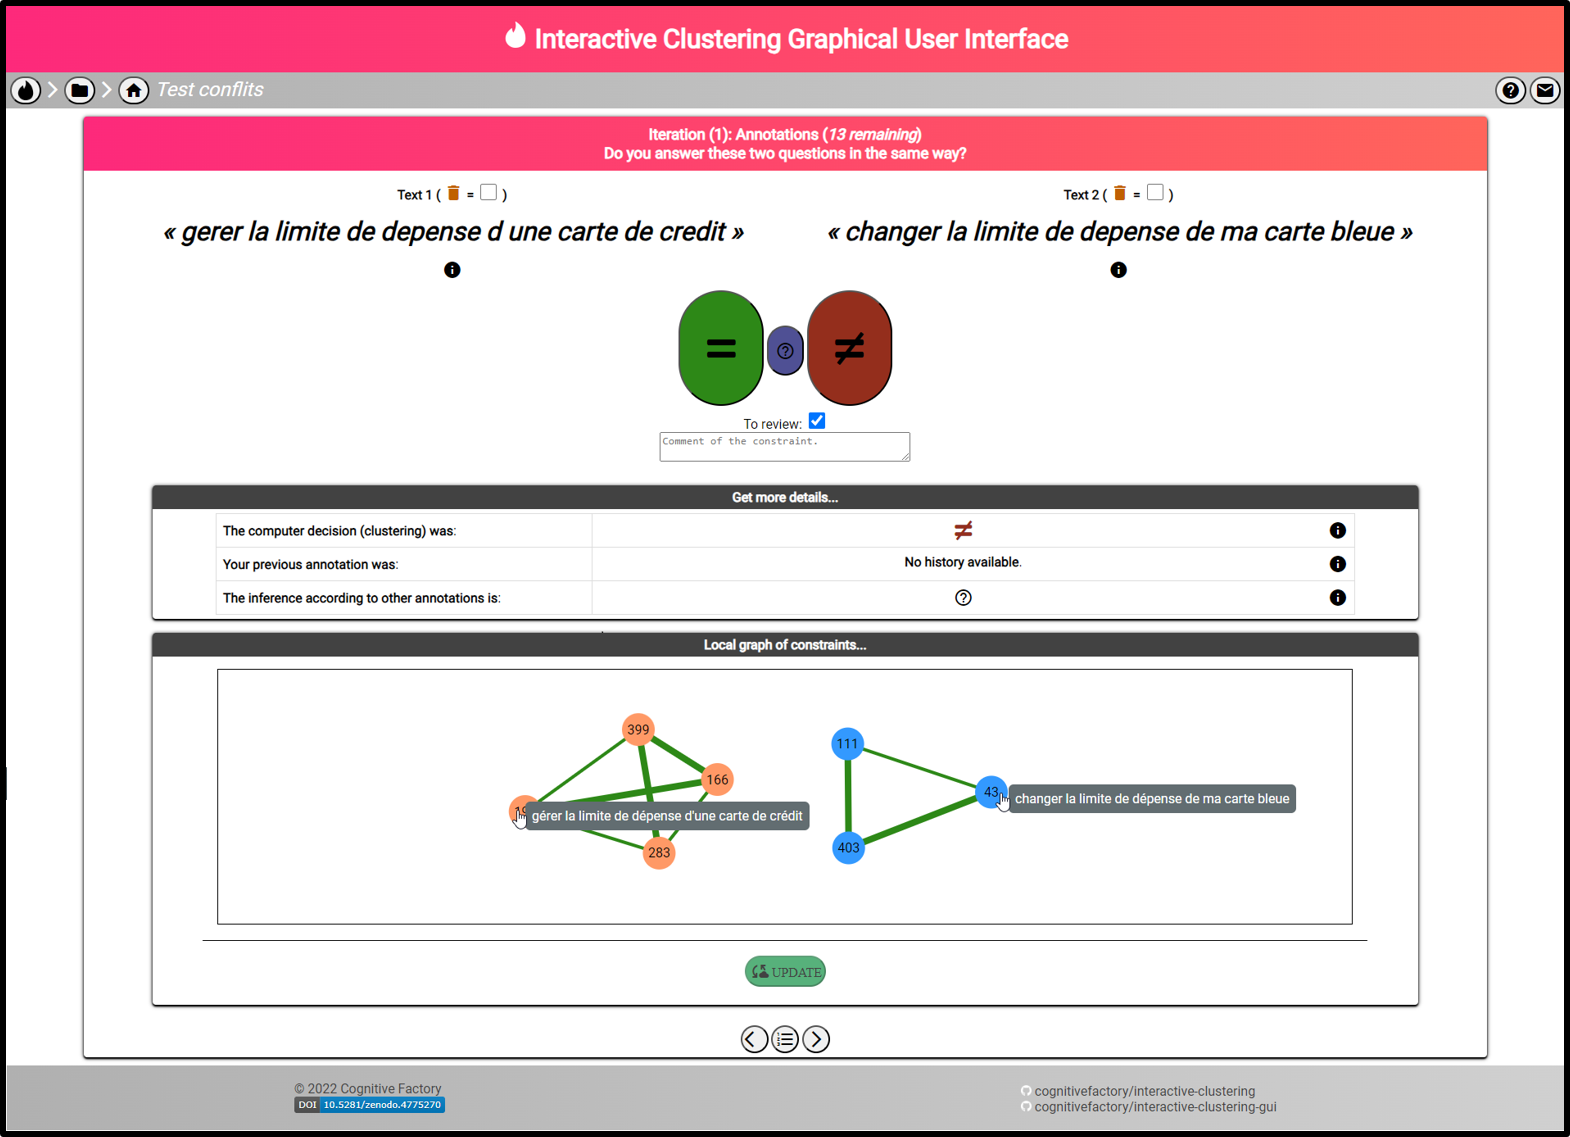
\includegraphics[width=0.95\textwidth]{figures/interactive-clustering-application-annotation-0full}
			\caption{
				Capture d'écran de l'application web implémentant notre méthodologie de \texttt{Clustering Interactif} : \textbf{page d'annotation d'une contrainte}.
			}
			\label{figure:C-WEB-APPLICATION-ANNOTATION}
		\end{figure}
		
		% Description générale.
		Cette page est le coeur de cette application d'annotation.
		\todo[inline]{à rédiger}
			% boutons d'annotation
			% boutons de revue et commentaire
			% détails
			% graphe de contraintes
			% cas de conflit
		
		% Capture d'écran: conflit d'annotation.
		\begin{figure}[H]
			\centering
			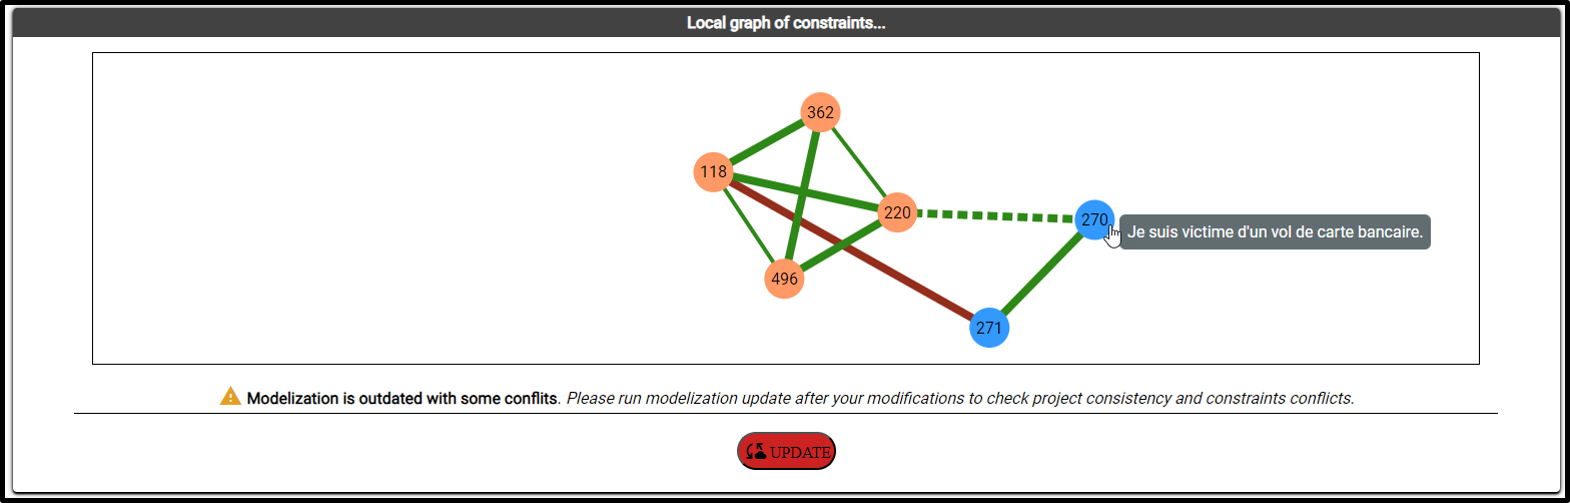
\includegraphics[width=0.95\textwidth]{figures/interactive-clustering-application-annotation-4conflit}
			\caption{
				Capture d'écran de l'application web implémentant notre méthodologie de \texttt{Clustering Interactif} : \textbf{graphe de contraintes présentant un conflit d'annotation}.
			}
			\label{figure:C-WEB-APPLICATION-CONFLIT}
		\end{figure}